

\documentclass[letter, 10pt, margins=0.3in]{texMemo}

\usepackage{amsmath}
\usepackage{booktabs}
\usepackage{color, soul}
\usepackage{dcolumn}
\usepackage{enumitem}

    \newcolumntype{d}[1]{D{.}{.}{#1}}
\usepackage[colorlinks=true, citecolor=blue]{hyperref}

\usepackage{graphicx, lipsum}

\usepackage{imakeidx}

\usepackage{caption}
\usepackage{subcaption}

\usepackage[LGRgreek]{mathastext}

\usepackage{listings}
\usepackage[]{matlab-prettifier}

\usepackage{multirow}

\usepackage{natbib}
\bibliographystyle{apalike}

\usepackage{printlen}  % \printlength\textwidth - To determine textwidth of document.  Here is it 496 pt.

\usepackage{siunitx}

\usepackage{tablefootnote}

\usepackage[table]{xcolor}
\definecolor{maroon}{cmyk}{0,0.87,0.68,0.32}
\definecolor{LightCyan}{rgb}{0.88,1,1}
\definecolor{Gray}{gray}{0.85}


\newcommand{\is}[1]{%
\if@noftnote%
\index{#1}%
\else%
\index{#1|fn{\number\value{footnote}}}%
\fi%
}

\makeindex


\graphicspath{ {../} }


\memodate{\today~(Submitted)}
\memosubject{Module 5 Assignment - Order Tracking of Mobius Propeller Data  \\}



\begin{document}

\maketitle


\vspace{-1.0cm}
\section*{Order Tracking of Mobius Propeller Data}


\vspace{-0.25cm}
The Matlab code for this problem is listed in Appendix~\ref{appendix:problem1}.


\vspace{-0.2cm}
\subsection*{Sound Pressure Level Versus Microphone Placement Angle}

\vspace{-0.2cm}
Figure~\ref{figure:1soundPressureLevelVersusMicrophonePlacementAngle} shows the sound pressure generated by the Mobius propeller versus the angle of microphone placement.

\vspace{-0.2cm}
\begin{figure}[htb!]
    \vspace{-0.1cm}
    \center
        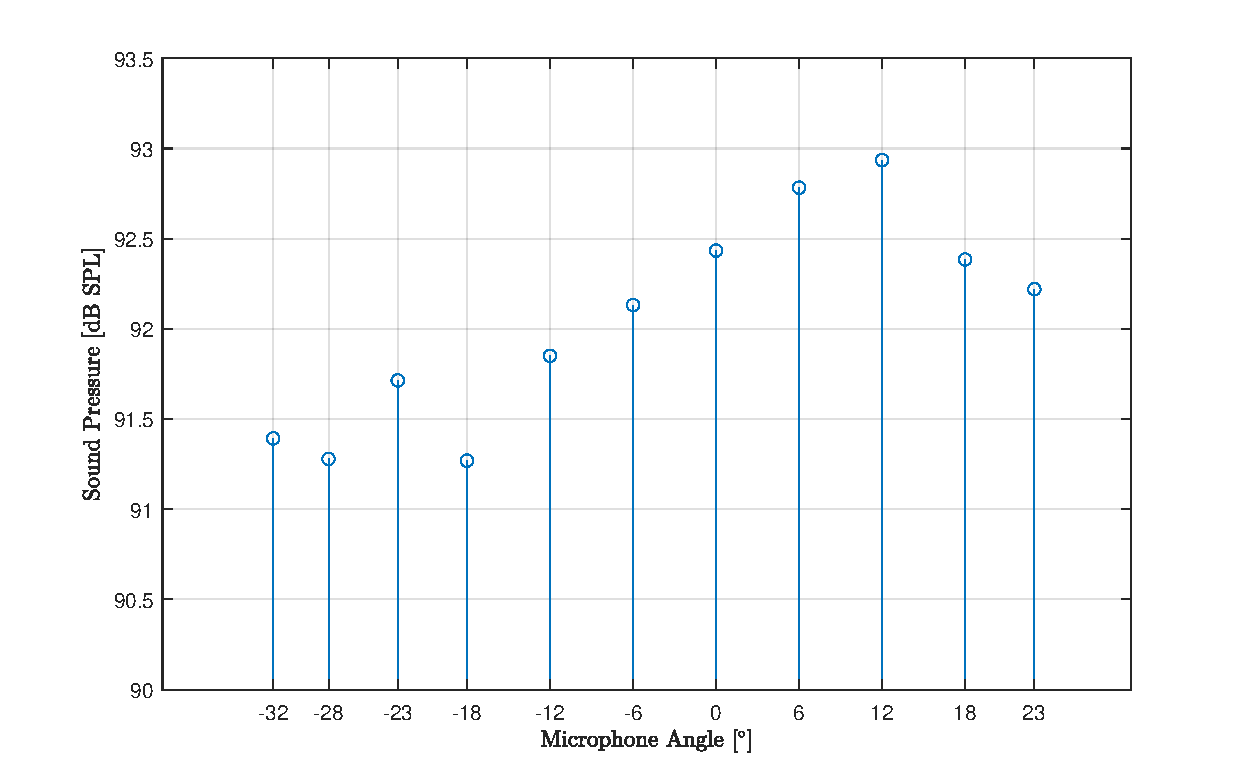
\includegraphics[scale = 0.6, keepaspectratio]{Sound Pressure Lever Versus Angle.pdf}
    \caption{Sound pressure level versus microphone placement angle.}
    \label{figure:1soundPressureLevelVersusMicrophonePlacementAngle}
\end{figure}

The highest sound pressure levels occur around the 0$^\circ$ plane, when the propeller is in the same plane as the microphone.  The highest sound pressure, approximately 93 dB SPL, occurs at 12$^\circ$, is radiated above the plane of the propeller and the drone itself.



\vspace{-0.2cm}
\subsection*{Trigger Signal and Representative Pressure Recording}

\vspace{-0.2cm}
Figure~\ref{figure:2triggerSignalAndAMicrophoneRecording} shows the angular position trigger signal and the pressure recording for a measurement angle of 0$^\circ$..

\vspace{-0.2cm}
\begin{figure}[htb!]
    \vspace{-0.1cm}
    \center
        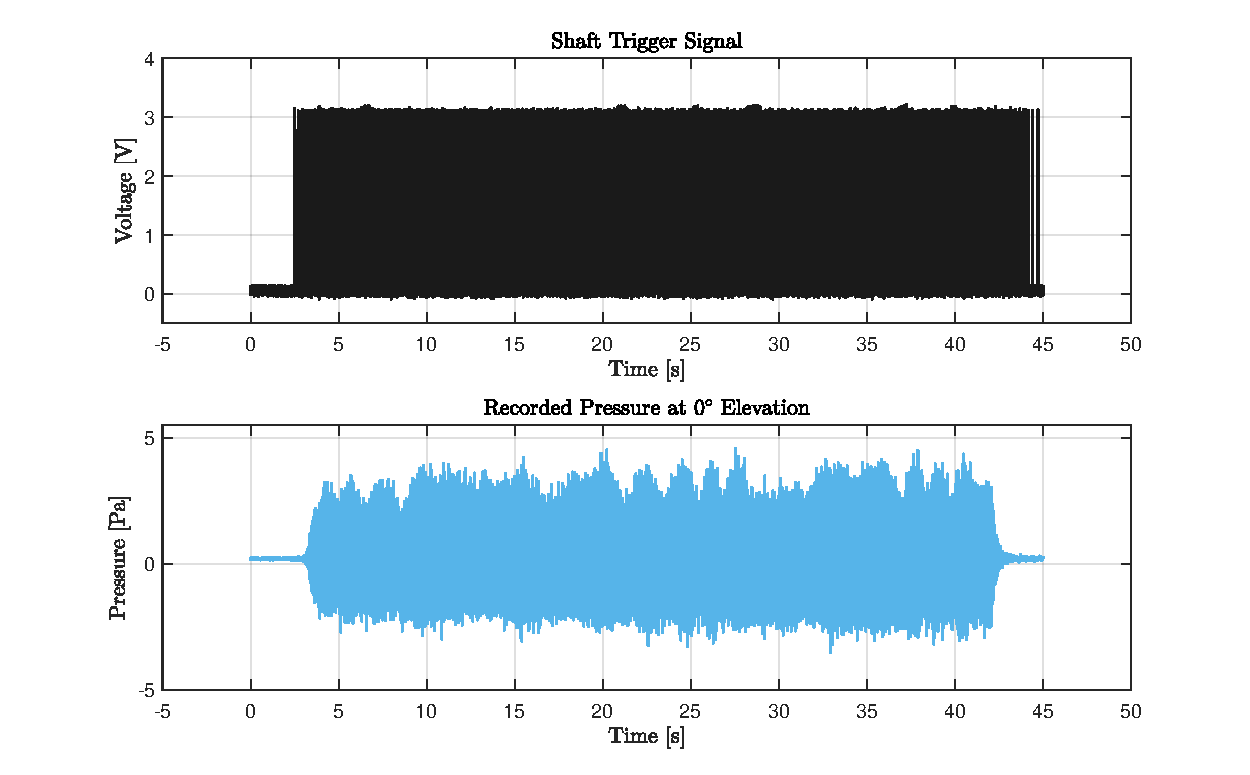
\includegraphics[scale = 0.6, keepaspectratio]{Trigger and a Microphone Pressure Recording.pdf}
    \caption{Trigger signal and a pressure recording at 0$^\circ$.}
    \label{figure:2triggerSignalAndAMicrophoneRecording}
\end{figure}



\vspace{-0.2cm}
\subsection*{Estimate of Shaft Rotation Speed}

\vspace{-0.2cm}
Figure~\ref{figure:4rpmEstimate} shows the estimate rotation speed of the shaft per revolution of the shaft.

\vspace{-0.2cm}
\begin{figure}[htb!]
    \vspace{-0.1cm}
    \center
        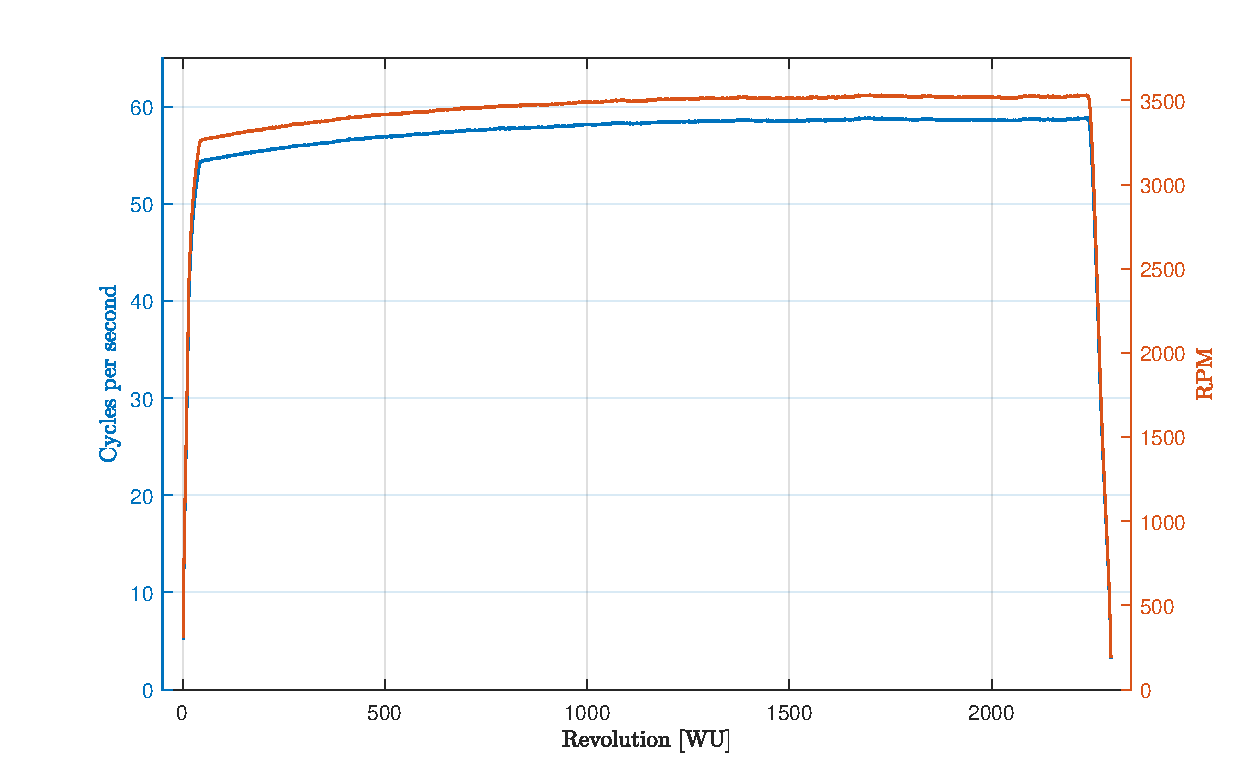
\includegraphics[scale = 0.7, keepaspectratio]{RPM Estimate.pdf}
    \caption{Rotation speed estimation.}
    \label{figure:4rpmEstimate}
\end{figure}

The maximum shaft rotation speed is approximately 58.9 cycles per second, or 3,532 RPM.  This maximum rotation speed occurs in revolution 1,672.



\vspace{-0.2cm}
\subsection*{Spectrogram of Recording at the 0$^\circ$ Recording Angle}

\vspace{-0.2cm}
Figure~\ref{figure:3spectrogram} shows the spectrogram for the pressure recording for a measurement angle of 0$^\circ$.

\vspace{-0.2cm}
\begin{figure}[htb!]
    \vspace{-0.1cm}
    \center
        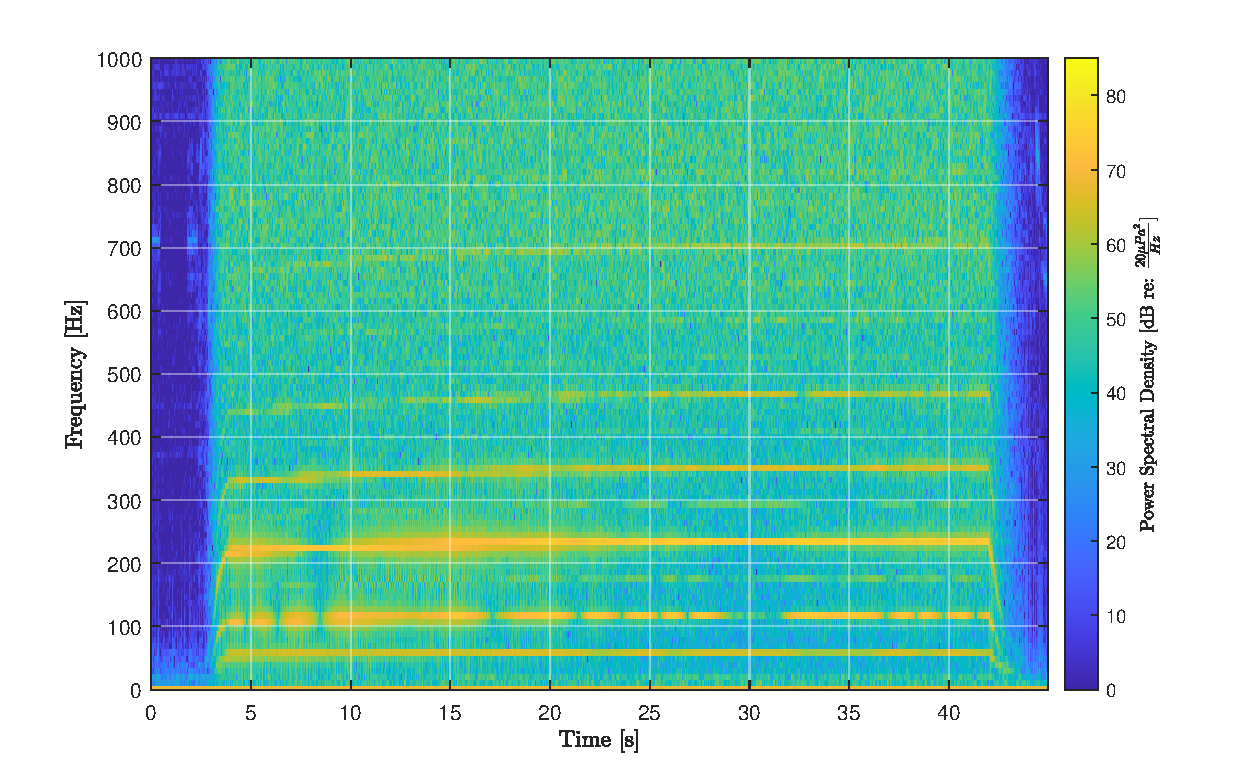
\includegraphics[scale = 0.7, keepaspectratio]{Spectrogram.pdf}
    \caption{Spectrogram for the pressure recording at 0$^\circ$.}
    \label{figure:3spectrogram}
\end{figure}

The bottom trace in the spectrogram, which corresponds to the shaft rotation, is about 58.6 cycles per second.








%track harmonics of shaft rate - ORDERS
%
%sample rate must be substantially higher than the maximum rotation rate of the shaft
%
%regions:  acceleration, steady-state, and deceleration





%\vspace{0.2cm}
%Table~\ref{table:1bLevels} lists the sound pressure levels for the 4 types of patterns for 1 kHz.
%
%\vspace{0.25cm}
%\setlength{\abovecaptionskip}{1.5pt}
%\vspace{0.1cm}
%{\renewcommand{\arraystretch}{1.5}
%\begin{table}[htpb!]
%    \footnotesize
%    \centering
%        \begin{tabular}{ | c | c | }
%        \hline
%        \textbf{Source Type}  &  \textbf{Sound Pressure Level [dB]}   \\
%        \hline
%        Monopole  &  58.6   \\
%        \hline
%        Dipole  &  61.6   \\
%        \hline
%        Lateral Quadrupole  &  48.2   \\
%        \hline
%        Linear Quadrupole  &  53.9  \\
%        \hline
%        \end{tabular}
%
%        \vspace{0.5cm}
%        \caption{Sound pressure levels for 1 kHz at 1 m distance.}
%        \label{table:1bLevels}
%
%\end{table}


%\vspace{0.25cm}
%The monopole had a volume velocity of 1.4 $\frac{m^3}{s}$.
%
%\vspace{0.25cm}
%The dipole had two equal strength, in-phase elements with a separation of 0.0429 $m$, which is less than the 1 $kHz$ wavelength of 0.343 $m$.  The volume velocity for both sources was 1.4 $\frac{m^3}{s}$.
%
%\vspace{0.25cm}
%The lateral quadrupole had four equal strength, diagonally opposite in-phase pairs with a separation of 0.0429 $m$.  The volume velocity for both sources was 1.4 $\frac{m^3}{s}$.
%
%\vspace{0.25cm}
%The linear quadrupole had three sources, the end sources were equal strength and in-phase, while the center source was twice the strength of the single sources and 180 $^\circ$ out-of-phase.  The separation between all three sources was 0.0429 $m$.  The volume velocity of the end sources was 1.4 $\frac{m^3}{s}$ and the volume velocity for the center source was 2.8 $\frac{m^3}{s}$.










\newpage
\section{Appendix - Matlab Code for Problem 1}
\label{appendix:problem1}

\lstinputlisting[style=Matlab-editor, numbers=left, mlshowsectionrules, basicstyle=\scriptsize]{../ACS_547_Module_5_Question_5_Sunday_April_20_2025.m}






\end{document}


% Reference(s):

% https://tex.stackexchange.com/questions/180222/how-to-change-font-size-for-specific-lstlisting









